\documentclass[a4paper]{article}

%% language and font encodings
\usepackage[english]{babel}
\usepackage[utf8x]{inputenc}
\usepackage[T1]{fontenc}

%% set page size and margins
\usepackage[a4paper,top=3cm,bottom=2cm,left=3cm,right=3cm,marginparwidth=1.75cm]{geometry}

%% define default sans font family for the document as roboto
%% sfdefault sets roboto as font for the main text
\usepackage[sfdefault, light, medium]{roboto}

\usepackage{float}						% package introducing floats like figure,...
\usepackage{listings}					% introduces source code listings with code highlighting
\usepackage{tikz}						% enables drawing awesome graphics directly with LaTex commands
\usetikzlibrary{arrows}					% tikz library for drawing arrows
\usepackage{xcolor}						% introduces lots of different (font) colors
\usepackage{amsmath}					% introduces most standard math environments and commands
\usepackage{graphicx}					% package needed to insert graphic objects like images
\usepackage[colorinlistoftodos]{todonotes} % introduces a simple method of inserting TODO notes in the document
\usepackage[colorlinks=true, allcolors=blue]{hyperref} % introduces hyperlinks in the document

%% styling of section titles
\usepackage{titlesec}
%% design for section and subsection headings
\titleformat{\section}[hang]{\normalfont\Large}{\thesection}{0.5em}{}[]
\titleformat{\subsection}[hang]{\normalfont\large}{\thesubsection}{0.5em}{}[]

%% define style of tikz nodes for drawing graphs
\tikzset{
  treenode/.style = {align=center, inner sep=8pt, text centered,
    font=\sffamily},
  arn_n/.style = {treenode, circle, black, draw=black,
    text width=1.5em},
}

%% define listing style for shell languages
\lstdefinestyle{myshell}{
  basicstyle=\small\ttfamily,
  numbers=none,
  frame=tblr,
  columns=fullflexible,
  backgroundcolor=\color{blue!10},
  linewidth=\linewidth
}

%% define a basic styling for a language listing e.g. for python (which is defined in the actual listing)
\lstset{
  backgroundcolor=\color{blue!10},  	% choose the background color
  basicstyle=\ttfamily,        			% size of fonts used for the code
  breaklines=true,                 		% automatic line breaking only at whitespace
  captionpos=b,                    		% sets the caption-position to bottom
  frame=tblr,
  commentstyle=\color{purple},    		% comment style
  keywordstyle=\color{blue},      		% keyword style
  stringstyle=\color{red},     			% string literal style
}

%% remove indents at the beginning of a paragraph in whole file
\setlength\parindent{0pt} 

%% specify, how many % floats have to make up in a page that the page becomes a float only page
\renewcommand{\floatpagefraction}{.8}%

% set title and author of the document
\title{This is the document title}
\author{This is the author of the document}

\begin{document}
\maketitle
\section{This is a section heading}
\label{sec:sectionheading}

The document is just a basic framework including enough functionality for most purposes.\newline

Lorem ipsum dolor sit amet, consetetur sadipscing elitr, sed diam nonumy eirmod tempor invidunt ut labore et dolore magna aliquyam erat, sed diam voluptua. At vero eos et accusam et justo duo dolores et ea rebum. Stet clita kasd gubergren, no sea takimata sanctus est Lorem ipsum dolor sit amet. Lorem ipsum dolor sit amet, consetetur sadipscing elitr, sed diam nonumy eirmod tempor invidunt ut labore et dolore magna aliquyam erat, sed diam voluptua. At vero eos et accusam et justo duo dolores et ea rebum. Stet clita kasd gubergren, no sea takimata sanctus est Lorem ipsum dolor sit amet.
\newline

\subsection{This is a subsection heading}
\label{subsec:subsectionheading}

Here comes a reference to an image: fig.\ \ref{fig:image}. And here one for a code listing: lst.\ \ref{lst:script_t1}.
\newline

This is a reference a a section: sec.\ \ref{sec:sectionheading}.\newline

\begin{lstlisting}[style=myshell, caption={This is a sample listing for shell commands.}, label={lst:mn_setup1},captionpos=b]
sudo mn --custom MyTopo.py --topo MyTopo --controller=remote,ip=127.0.0.1,port=6633 --switch ovsk,protocols=OpenFlow13 --link tc
\end{lstlisting}

\begin{lstlisting}[language=Python, caption={Note that the shown code does not necessarily make sense ;-). Shows listing in Python.},label={lst:script_t1},captionpos=b]
  #!/usr/bin/python
  from  mininet.net   import Mininet

  class MyTopo( Topo ) :
      def __init__( self ) :
          # parent  class  Topo  initialization
          Topo.__init__( self )
          # Add hosts
          h1 = self.addHost ( 'h1', ip='172.31.1.1/24' )
          # Add switches
          s1 = self.addSwitch( 's1' )
          # Add links
          self.addLink( h1 , s1 , bw=100 )      
  topos = {'MyTopo':  (  lambda : MyTopo() )}

\end{lstlisting}

This is an example for a url:  \url{https://github.com/rkoenigstein}.\clearpage

Here comes a figure.\newline

\begin{figure}[htbp]
	\centering
	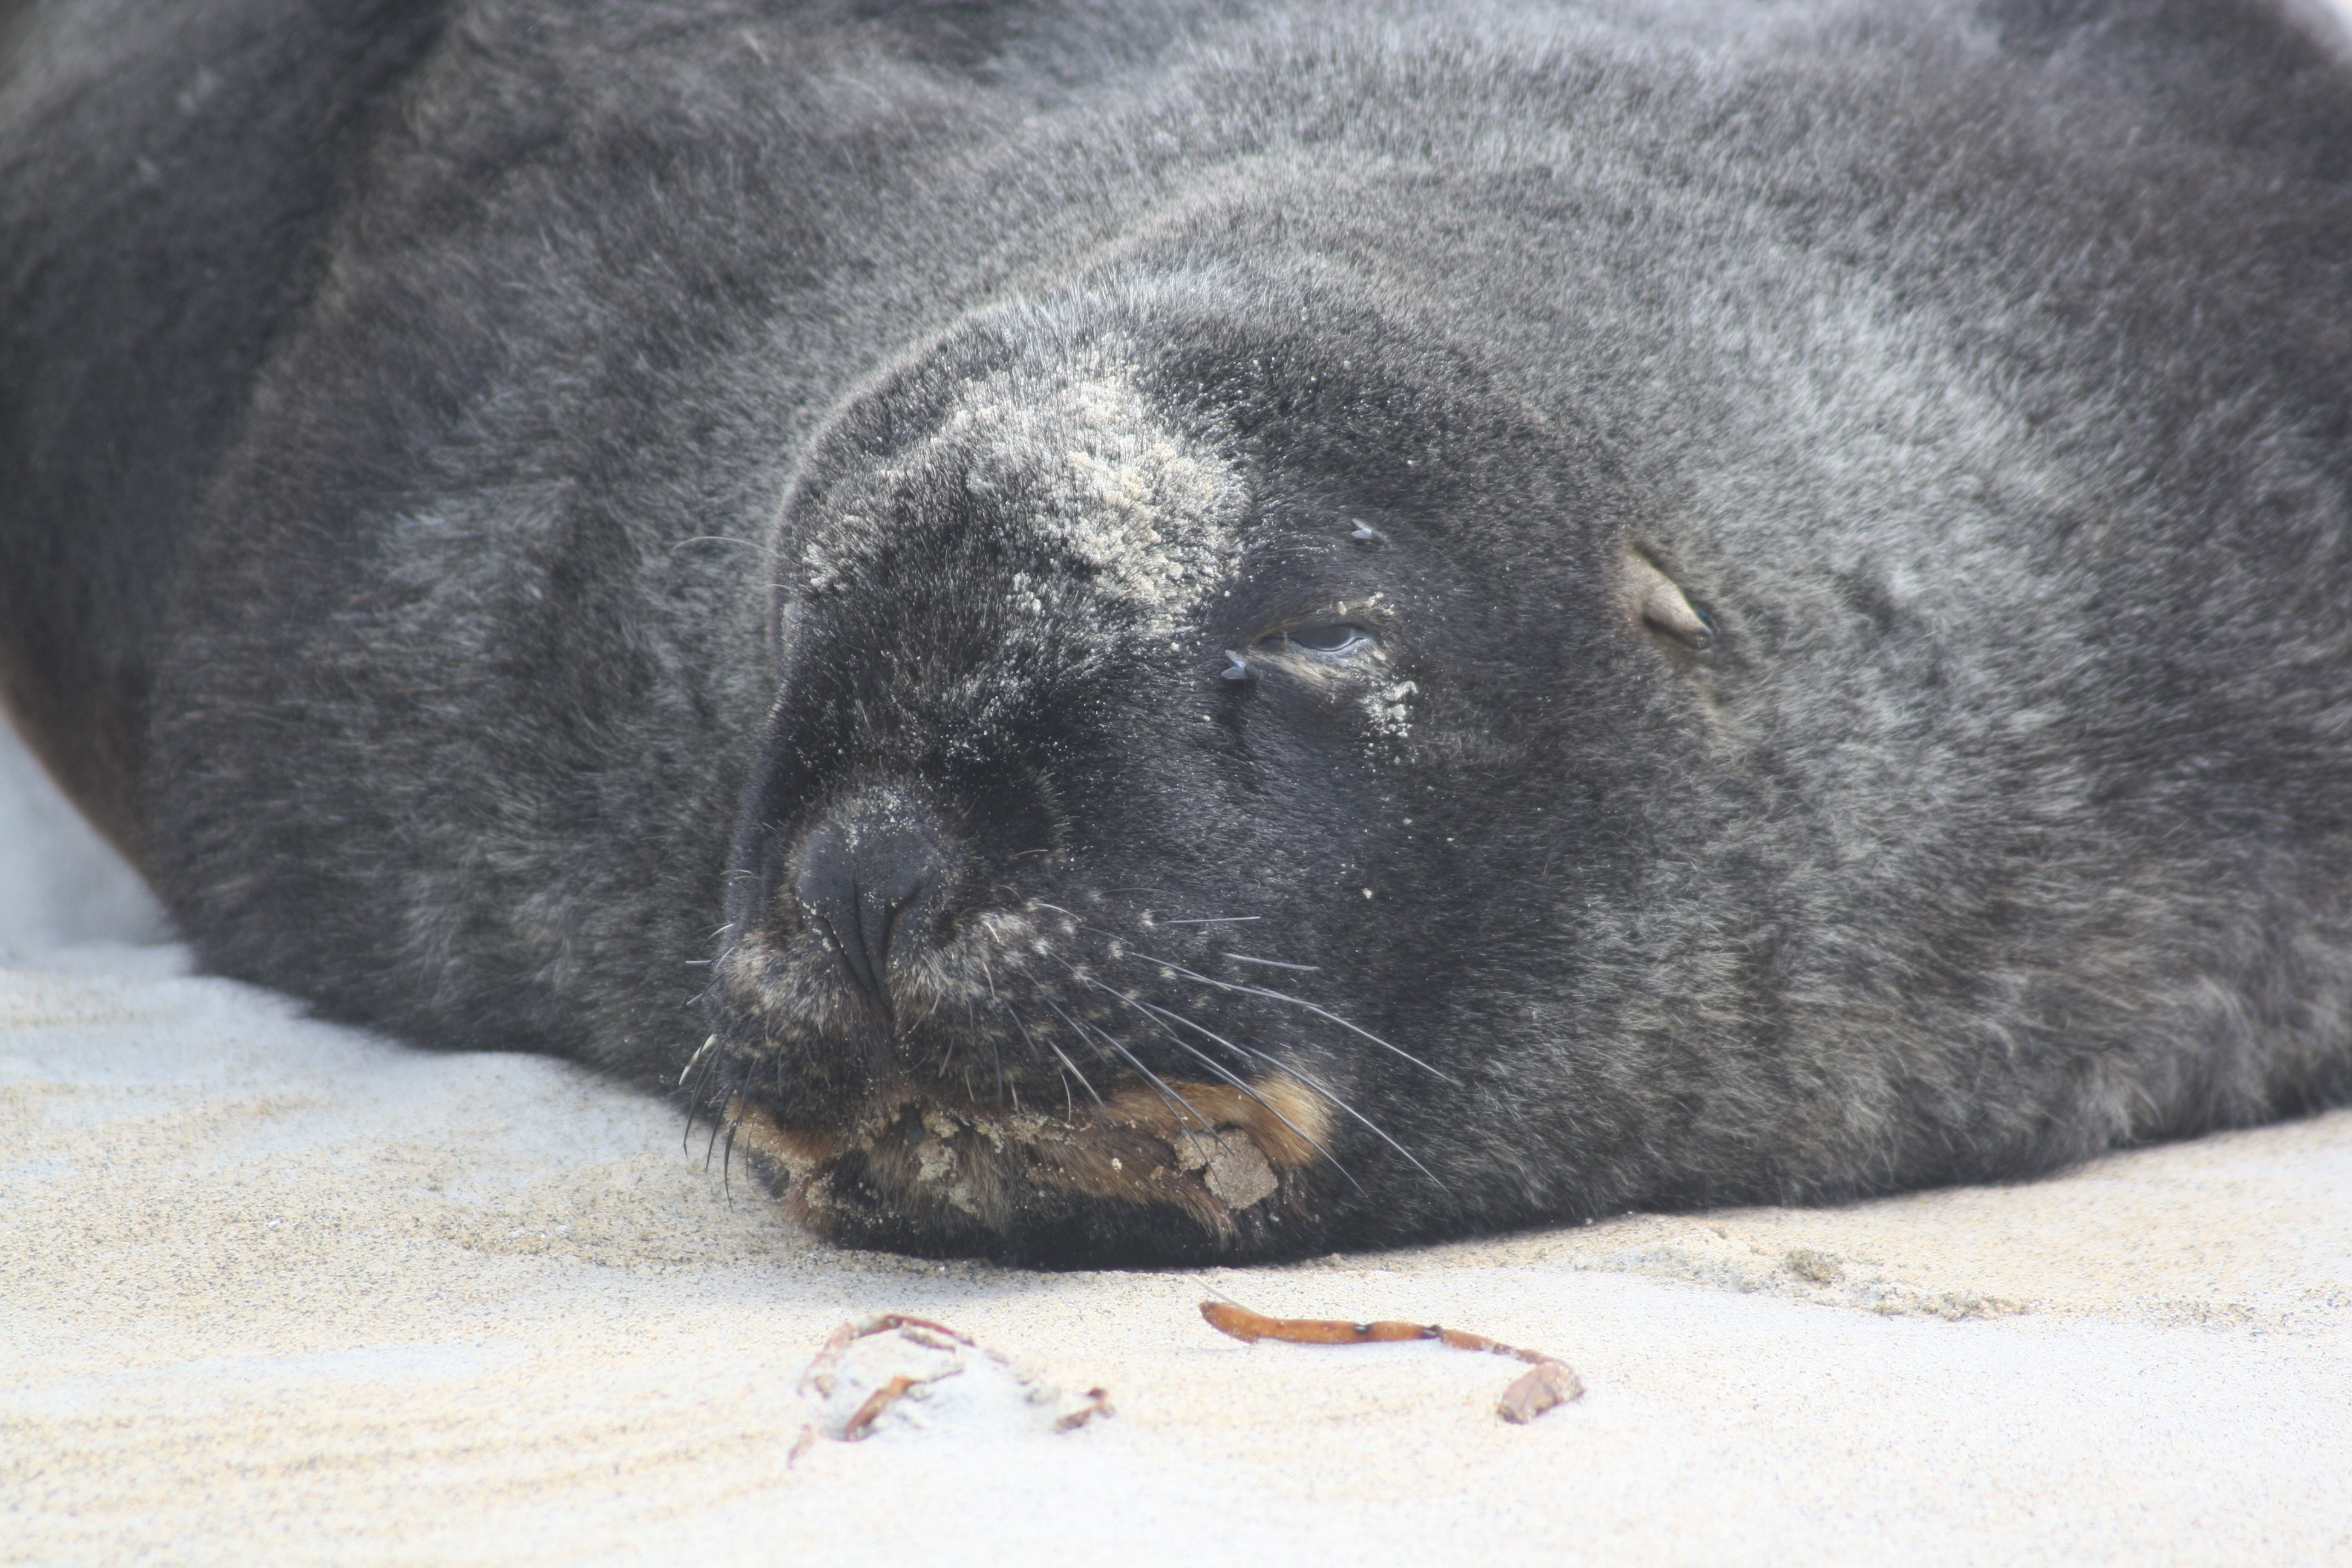
\includegraphics[width=1\textwidth]{sealion.jpg}
	\caption{Second SDN to be created}
	\label{fig:image}
\end{figure}

Here comes a graph generated with tikz:\newline

\begin{figure}[htbp]
  \centering
  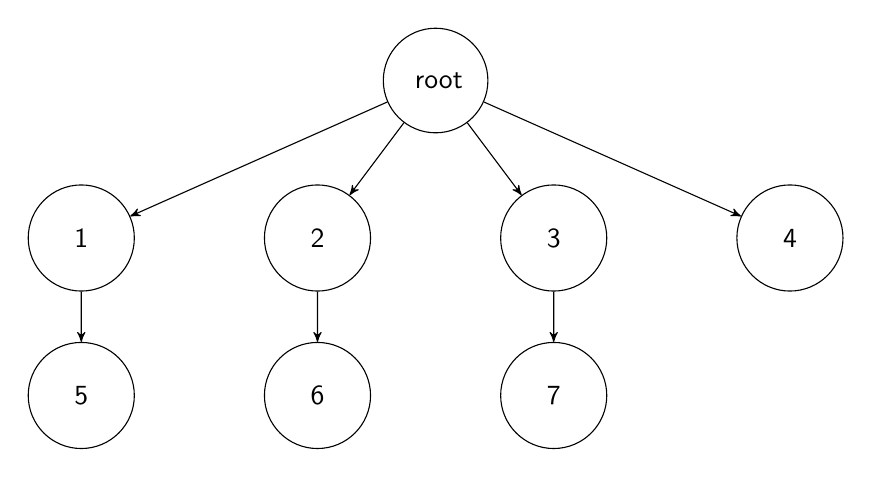
\begin{tikzpicture}[->,>=stealth',level/.style={sibling distance = 3cm/#1,
    level distance = 2cm}]
  \node [arn_n] {root}
      child{ node [arn_n] {1}
          child{ node [arn_n] {5}
          }
          }
      child{ node [arn_n] {2}
          child{ node [arn_n] {6}
          }
          }
      child{ node [arn_n] {3}
          child{ node [arn_n] {7}
          }
          }
      child{ node [arn_n] {4}
          }
  ;
  \end{tikzpicture}
  \caption{Basic graph generated with the tikz package.}
  \label{fig:tikz_graph}
\end{figure}

\end{document}
